% Ubah judul dan label berikut sesuai dengan yang diinginkan.
\section{Result and Discussion}
\label{sec:resultanddiscussion}

% Ubah paragraf-paragraf pada bagian ini sesuai dengan yang diinginkan.
\subsection{Model Performance Testing using Confusion Matrix}

In this research, the Convolutional Neural Network (CNN) method is used to create a model. During CNN model building, image data is collected and grouped which is then used as a dataset for CNN model training and validation. The data trained in the form of eye landmark images that have been grouped into five classes as described in the methodology. The five classes that classify the eye landmark image data are “Right” (\emph{"Kanan"}), “Left” (\emph{"Kiri"}), “Forward” (\emph{"Maju"}), “Backward” (\emph{"Mundur"}), and “Stop”. The dataset used in this research consists of 2000 image data. Furthermore, in each class folder, the 400 image data is divided (split) with a weight of 70\% for training data so that there are 280 image data entered in the training folder and 30\% weight for validation data so that there are 120 image data entered in the validation folder. The visualization of the dataset used can be seen in Figure \ref{fig:dataset}.

\begin{figure} [ht] \centering
  % Nama dari file gambar yang diinputkan
  \includegraphics[scale=0.38]{gambar/bab4/visual.png}
  % Keterangan gambar yang diinputkan
  \caption{Dataset Visual Diagram}
  % Label referensi dari gambar yang diinputkan
  \label{fig:dataset}
\end{figure}

In model building, the training process is carried out using a CNN model consisting of eleven layers with 32 filters in the first layer, 64 filters in the second layer, and 128 filters in the third layer as the structure described in the research methodology. Training on the CNN model is done with a configuration of 40 epoch stages with 10 training steps per epoch. The early stopping module is also added during model training in order to obtain the best model, which is at the 30th epoch. Based on the training results, an accuracy value of 100\% is generated with a validation accuracy of 99.83\%. In addition, the training results also show a loss value of 0.22\% with a validation loss of 1.14\%. These variables can be seen in Figure \ref{fig:acc_loss} which has visualized the results of accuracy and validation accuracy as well as the results of loss and loss validation in graphical form with the values of accuracy, validation accuracy, loss, and loss validation against each stage of epoch.

\begin{figure}[H]
  \centering
  \subfloat[Accuracy]{
    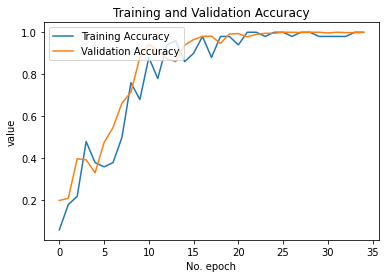
\includegraphics[width=0.23\textwidth]{gambar/bab4/model5 (30cm)/train.png}
    %\caption{30 sentimeter}
    \label{fig:imageaccu}}
    \hfil 
  \subfloat[Loss]{
    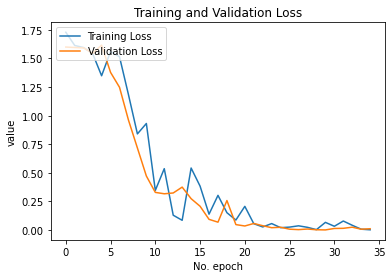
\includegraphics[width=0.23\textwidth]{gambar/bab4/model5 (30cm)/loss.png}
    %\caption{50 sentimeter}
    \label{fig:imageloss}}

  \caption{Graph of Accuracy and Loss on the Model Training Results}
  \label{fig:acc_loss}
\end{figure}

After obtaining the accuracy and loss for the model training results, the next calculation is done for confusion matrix. The confusion matrix is calculated by comparing the actual label (true label) with the predicted label and then the two labels will be visualized into a matrix divided into each control class, where predicted label becomes the X-axis and true label becomes the Y-axis. From the visualization of confusion matrix from Figure \ref{fig:confuse}, it can be observed that there is a prediction error in the “Forward"  (\emph{"Maju"}) class.

\begin{figure} [H] \centering
  % Nama dari file gambar yang diinputkan
  \includegraphics[scale=0.5]{gambar/bab4/modelkedua/modelkedua.png}
  % Keterangan gambar yang diinputkan
  \caption{Model Confusion Matrix}
  % Label referensi dari gambar yang diinputkan
  \label{fig:confuse}
\end{figure}

Then from confusion matrix, we get classification results that can be grouped into several parameters, namely true positive, true negative, false positive, and false negative. True positive is the result where the model correctly predicts the positive class. Similarly, true negative is the result where the model correctly predicts the negative class. The positive class is the class itself, while the negative class is any class other than itself. False positive is the result where the model incorrectly predicts the positive class. And false negative is the result where the model incorrectly predicts the negative class. The classification results can be seen in Table \ref{tb:cm_model}.

%Tabel 4.2
\begin{table}[H]
  \caption{Model Validation Results}
  \label{tb:cm_model} 
  \centering
  \begin{tabular}{|l|c|c|c|c|}
  \hline
  \rowcolor[HTML]{C0C0C0} 
  \textbf{Class} & \textbf{TP} & \textbf{TN} & \textbf{FP} & \textbf{FN} \\ \hline
  Right    & 120          & 479         & 1           & 0           \\ \hline
  Left      & 120          & 480         & 0           & 0           \\ \hline
  Forward      & 119          & 480         & 0           & 1           \\ \hline
  Backward     & 120          & 480         & 0           & 0           \\ \hline
  Stop  & 120          & 480         & 0           & 0           \\ \hline
  \end{tabular}
\end{table}

From the classification results, the model validation value can then be calculated. The validation values calculated are accuracy, precision, recall, and f-1 score. A more detailed description can be seen in Table \ref{tb:vs_model}. It can be seen that the model has a high average accuracy value of 99.93\% with an average precision value of 99.83\%, average recall of 99.83\%, and average f-1 score of 99.83\%. This indicates that the model has a high level of accuracy in predicting eye poses.

%Tabel 4.3
\begin{table}[H]
  \caption{Model Validation Results}
  \label{tb:vs_model} 
  \centering
  \begin{tabular}{|l|c|c|c|c|}
  \hline
  \rowcolor[HTML]{C0C0C0} 
  \textbf{Class} & \textbf{Accuracy} & \textbf{Precision} & \textbf{Recall} & \textbf{F1-Score} \\ \hline
  Right    & 99.83\%            & 99.17\%             & 100\%           & 99.59\%            \\ \hline
  Left     & 100\%          & 100\%           & 100\%           & 100\%           \\ \hline
  Forward      & 99.83\%          & 100\%           & 99.17\%          & 99.58\%          \\ \hline
  Backward     & 100\%            & 100\%             & 100\%           & 100\%            \\ \hline
  Stop  & 100\%            & 100\%             & 100\%           & 100\%            \\ \hline
  \end{tabular}
\end{table}

\subsection{Model Performance Testing using Distance Variations}

In this test scenario, the model is tested based on several distance variations. Distance testing is useful to determine the performance and accuracy of the model if the input image is taken from different distances. This needs to be tested because the further the distance of the image detector, the smaller the visual image data obtained. The distance validation results used are 30 centimeters which can be seen in Table \ref{tb:30cm}, 50 centimeters in Table \ref{tb:50cm}, 70 centimeters in Table \ref{tb:70cm}, and 90 centimeters in Table \ref{tb:90cm}. For an example of the distance test variation dataset can be seen in Figure \ref{fig:Variasi Jarak Kamera}.

\begin{figure}[H]
  \centering
  \subfloat[30 centimeters]{
    
\includegraphics[width=0.2\textwidth]{gambar/bab4/30.jpg}
    %\caption{30 sentimeter}
    \label{fig:imagea}}
    \hfil 
  \subfloat[50 centimeters]{
    
\includegraphics[width=0.2\textwidth]{gambar/bab4/50.jpg}
    %\caption{50 sentimeter}
    \label{fig:imageb}}

  \subfloat[70 centimeters]{
    
\includegraphics[width=0.2\textwidth]{gambar/bab4/70.jpg}
    %\caption{70 sentimeter}
    \label{fig:imagec}}
    \hfil
  \subfloat[90 centimeters]{
    
\includegraphics[width=0.2\textwidth]{gambar/bab4/90.jpg}
    %\caption{90 sentimeter}
    \label{fig:imaged}}

  \caption{Camera Distance Variations}
  \label{fig:Variasi Jarak Kamera}
\end{figure}

\begin{table}[ht]
  \caption{Model Validation Results with a Distance of 30 cm}
  \label{tb:30cm}
  \centering
  \begin{tabular}{|l|c|c|c|c|}
  \hline
  \rowcolor[HTML]{C0C0C0} 
  \textbf{Class} & \textbf{Accuracy} & \textbf{Precision} & \textbf{Recall} & \textbf{F1-Score} \\ \hline
  Right    & 100\%            & 100\%             & 100\%           & 100\%            \\ \hline
  Left     & 100\%          & 100\%           & 100\%           & 100\%           \\ \hline
  Forward      & 100\%          & 100\%           & 100\%          & 100\%          \\ \hline
  Backward     & 100\%            & 100\%             & 100\%           & 100\%            \\ \hline
  Stop  & 100\%            & 100\%             & 100\%           & 100\%            \\ \hline
  \end{tabular}
\end{table}

\begin{table}[ht]
  \caption{Model Validation Results with a Distance of 50 cm}
  \label{tb:50cm}
  \centering
  \begin{tabular}{|l|c|c|c|c|}
  \hline
  \rowcolor[HTML]{C0C0C0} 
  \textbf{Class} & \textbf{Accuracy} & \textbf{Precision} & \textbf{Recall} & \textbf{F1-Score} \\ \hline
  Right    & 100\%            & 100\%             & 100\%           & 100\%            \\ \hline
  Left     & 100\%          & 100\%           & 100\%           & 100\%           \\ \hline
  Forward      & 100\%          & 100\%           & 100\%          & 100\%          \\ \hline
  Backward     & 100\%            & 100\%             & 100\%           & 100\%            \\ \hline
  Stop  & 100\%            & 100\%             & 100\%           & 100\%            \\ \hline
  \end{tabular}
\end{table}

\begin{table}[H]
  \caption{Model Validation Results with a Distance of 70 cm}
  \label{tb:70cm}
  \centering
  \begin{tabular}{|l|c|c|c|c|}
  \hline
  \rowcolor[HTML]{C0C0C0} 
  \textbf{Class} & \textbf{Accuracy} & \textbf{Precision} & \textbf{Recall} & \textbf{F1-Score} \\ \hline
  Right    & 100\%            & 100\%             & 100\%           & 100\%            \\ \hline
  Left     & 100\%          & 100\%           & 100\%           & 100\%           \\ \hline
  Forward      & 99.50\%          & 100\%           & 97.50\%          & 98.73\%          \\ \hline
  Backward     & 99.50\%            & 97.56\%             & 100\%           & 98.77\%            \\ \hline
  Stop  & 100\%            & 100\%             & 100\%           & 100\%            \\ \hline
  \end{tabular}
\end{table}

\begin{table}[H]
  \caption{Model Validation Results with a Distance of 90 cm}
  \label{tb:90cm}
  \centering
  \begin{tabular}{|l|c|c|c|c|}
  \hline
  \rowcolor[HTML]{C0C0C0} 
  \textbf{Class} & \textbf{Accuracy} & \textbf{Precision} & \textbf{Recall} & \textbf{F1-Score} \\ \hline
  Right    & 100\%            & 100\%             & 100\%           & 100\%            \\ \hline
  Left     & 100\%          & 100\%           & 100\%           & 100\%           \\ \hline
  Forward      & 96.67\%          & 94.64\%           & 88.33\%          & 91.38\%          \\ \hline
  Backward     & 96.67\%            & 89.06\%             & 95\%           & 91.94\%            \\ \hline
  Stop  & 100\%            & 100\%             & 100\%           & 100\%            \\ \hline
  \end{tabular}
\end{table}
    
\subsection{Model Performance Testing using Lighting Variations}

In eye pose-based wheelchair control systems, lighting variations have a significant influence on the performance of the detection model. The purpose of this test is to evaluate the success and failure rate of the model in detecting eye poses in three lighting conditions, such as dark lighting (35 Lux) which can be seen in Table \ref{tb:lux35}, dim (55 Lux) in Table \ref{tb:lux55}, and bright (131 Lux) in Table \ref{tb:lux131}. The type of lighting tested was ambient light, which simulates ambient lighting with different intensity variations. For lighting test variations can be seen in Figure \ref{fig:Variasi Pencahayaan}.

\begin{figure}[H]
  \centering
  \subfloat[35 Lux]{
    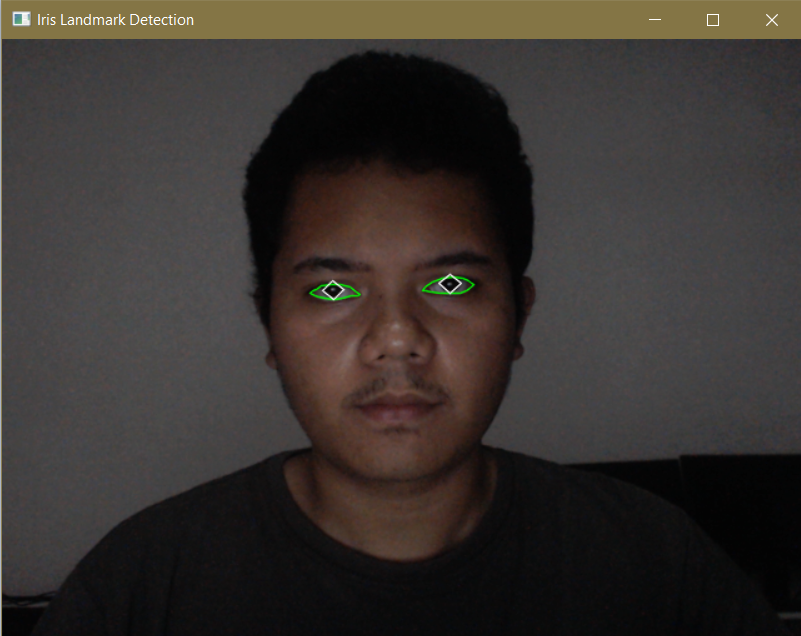
\includegraphics[width=0.15\textwidth]{gambar/bab4/33.png}
    %\caption{30 sentimeter}
    \label{fig:imageaa}}
  \hfil
  \subfloat[55 Lux]{
    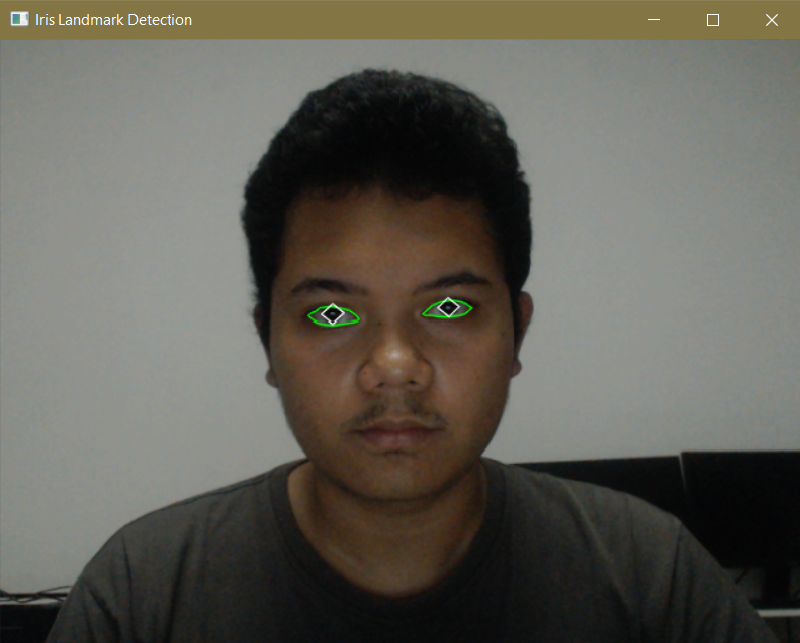
\includegraphics[width=0.15\textwidth]{gambar/bab4/55.png}
    %\caption{50 sentimeter}
    \label{fig:imagebb}}

  \subfloat[131 Lux]{
    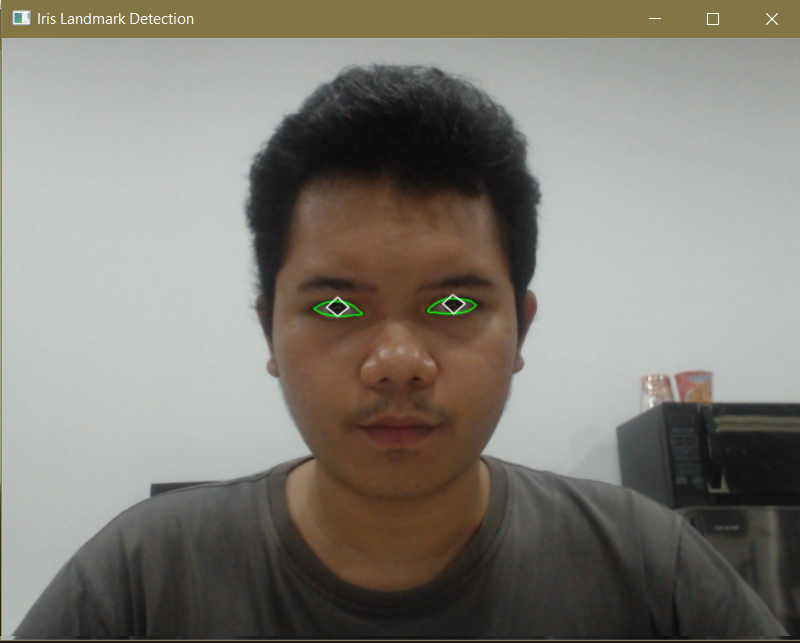
\includegraphics[width=0.15\textwidth]{gambar/bab4/131.png}
    %\caption{70 sentimeter}
    \label{fig:imagecc}}

  \caption{Lighting Variations}
  \label{fig:Variasi Pencahayaan}
\end{figure}

\begin{table}[ht]
  \caption{Model Testing with 35 Lux Lighting}
  \label{tb:lux35} 
  \centering
  \begin{tabular}{|l|c|c|}
  \hline
  \rowcolor[HTML]{C0C0C0} 
  \textbf{Class} &  \multicolumn{1}{c|}{\textbf{\begin{tabular}[c]{@{}c@{}}Percentage of  \\ Success\end{tabular}}} & \multicolumn{1}{c|}{\textbf{\begin{tabular}[c]{@{}c@{}}Percentage of\\ Unsuccess\end{tabular}}} \\ \hline
  Right                                                                                                                                                                             & 100\%                                                                                   & 0\%                                                                                         \\ \hline
  Left                                                                                                                                                                               & 100\%                                                                                   & 0\%                                                                                         \\ \hline
  Forward                                                                                                                                                                              & 90\%                                                                                    & 10\%                                                                                        \\ \hline
  Backward                                                                         & 93.33\%                                                                                 & 6.67\%                                                                                      \\ \hline
  Stop                                                                                          & 100\%                                                                                   & 0\%                                                                                         \\ \hline
\end{tabular}
\end{table}

\begin{table}[ht]
  \caption{Model Testing with 55 Lux Lighting}
  \label{tb:lux55} 
  \centering
  \begin{tabular}{|l|c|c|}
  \hline
  \rowcolor[HTML]{C0C0C0} 
  \textbf{Class} &  \multicolumn{1}{c|}{\textbf{\begin{tabular}[c]{@{}c@{}}Percentage of  \\ Success\end{tabular}}} & \multicolumn{1}{c|}{\textbf{\begin{tabular}[c]{@{}c@{}}Percentage of\\ Unsuccess\end{tabular}}} \\ \hline
  Right                                                                                                                                                                             & 100\%                                                                                   & 0\%                                                                                         \\ \hline
  Left                                                                                                                                                                               & 100\%                                                                                   & 0\%                                                                                         \\ \hline
  Forward                                                                                                                                                                              & 96.67\%                                                                                    & 3.33\%                                                                                        \\ \hline
  Backward                                                                         & 93.33\%                                                                                 & 6.67\%                                                                                      \\ \hline
  Stop                                                                                          & 100\%                                                                                   & 0\%                                                                                         \\ \hline
\end{tabular}
\end{table}

\begin{table}[H]
  \caption{Model Testing with 131 Lux Lighting}
  \label{tb:lux131} 
  \centering
  \begin{tabular}{|l|c|c|}
  \hline
  \rowcolor[HTML]{C0C0C0} 
  \textbf{Class} &  \multicolumn{1}{c|}{\textbf{\begin{tabular}[c]{@{}c@{}}Percentage of  \\ Success\end{tabular}}} & \multicolumn{1}{c|}{\textbf{\begin{tabular}[c]{@{}c@{}}Percentage of\\ Unsuccess\end{tabular}}} \\ \hline
  Right                                                                                                                                                                             & 100\%                                                                                   & 0\%                                                                                         \\ \hline
  Left                                                                                                                                                                               & 100\%                                                                                   & 0\%                                                                                         \\ \hline
  Forward                                                                                                                                                                              & 100\%                                                                                    & 0\%                                                                                        \\ \hline
  Backward                                                                         & 100\%                                                                                 & 0\%                                                                                      \\ \hline
  Stop                                                                                          & 100\%                                                                                   & 0\%                                                                                         \\ \hline
\end{tabular}
\end{table}

\subsection{Frame Per Second (FPS) Performance Testing on Wheelchair Control System}

The Frame Per Second (FPS) performance test aims to evaluate the speed of the system in processing eye poses in real-time to control the wheelchair. FPS is an important indicator in assessing the smoothness and responsiveness of the system, especially in applications that require pose detection and fast decision making. The FPS test results on the laptop and NUC can be seen in Table \ref{tb:fps}.

\begin{table}[H]
  \caption{FPS Performance Results on Laptop and NUC}
  \label{tb:fps}
  \centering
  \begin{tabular}{|l|c|c|}
  \hline
  \rowcolor[HTML]{C0C0C0} 
  \textbf{Class} &  \multicolumn{1}{c|}{\textbf{\begin{tabular}[c]{@{}c@{}}Average \\ FPS on Laptop\end{tabular}}} & \multicolumn{1}{c|}{\textbf{\begin{tabular}[c]{@{}c@{}}Average\\ FPS on NUC\end{tabular}}} \\ \hline
  Right           & 12.745              & 10.567           \\ \hline
  Left           & 12.635              & 10.617            \\ \hline
  Forward           & 13.078              & 10.068           \\ \hline
  Backward           & 13.507              & 9.734           \\ \hline
  Stop           & 12.580              & 10.127            \\ \hline
  \end{tabular}
\end{table}

\subsection{Inference Time on Model and Response Time on Wheelchair Motor Testing}

The Inference Time test on the model and Response Time test on the wheelchair motor aim to evaluate how fast the eye pose-based wheelchair control system can respond to commands from the user. Inference Time measures the time taken by the model to detect and classify eye poses, while Response Time measures the time taken for the wheelchair motor to start moving after receiving a signal from the model. The time test results of Inference Time and Response Time can be seen in Table \ref{tb:response}.

\begin{table}[H]
  \caption{Inference Time and Response Time Testing Results}
  \label{tb:response}
  \centering
  \begin{tabular}{|l|c|c|}
  \hline
  \rowcolor[HTML]{C0C0C0} 
  \textbf{Class} &  \multicolumn{1}{c|}{\textbf{\begin{tabular}[c]{@{}c@{}}Average \\ Inference Time (s)\end{tabular}}} & \multicolumn{1}{c|}{\textbf{\begin{tabular}[c]{@{}c@{}}Average\\ Response Time (s)\end{tabular}}} \\ \hline
  Right           & 0.0626             & 0.2328           \\ \hline
  Left           & 0.0640              & 0.0933            \\ \hline
  Forward           & 0.0656               & 0.4337           \\ \hline
  Backward           & 0.0637              & 0.1409           \\ \hline
  Stop           & 0.0666              & 0.4318            \\ \hline
  \end{tabular}
\end{table}

\subsection{Stability of Wheelchair Motor Testing}

The stability test on the wheelchair motor aims to ensure that the output time executed by the motor remains stable for each input given by the user through the eye pose control system. This involves measuring the time taken by the motor to respond to each eye pose command and ensuring that the response time remains consistent across different input conditions. The results of the motor stability test can be seen in Table \ref{tb:stabil}.

\begin{table}[H]
  \caption{Motor Stability Testing Results}
  \label{tb:stabil}
  \centering
  \begin{tabular}{|l|c|c|}
  \hline
  \rowcolor[HTML]{C0C0C0} 
  \textbf{Class} &  \multicolumn{1}{c|}{\textbf{\begin{tabular}[c]{@{}c@{}}Average \\ Motor Running Time (s)\end{tabular}}} \\ \hline
  Right          & 6.013                        \\ \hline
  Left           & 6.469                          \\ \hline
  Forward           & 6.532                         \\ \hline
  Backward         & 6.863                         \\ \hline
  Stop           & 4.933                          \\ \hline
  \end{tabular}
\end{table}